\documentclass[preprint,3p,number]{elsarticle}

\usepackage{amsmath}
\usepackage{amssymb}
\usepackage{subcaption}
% \usepackage{hyperref}
\usepackage{graphicx}
\usepackage{tikz}
\usepackage{pgfplots}
\usepackage{booktabs}
\usepackage{siunitx}
\usepackage[noabbrev,capitalize]{cleveref}
\usepackage{lipsum}

% Tikz libraries
\usetikzlibrary{arrows.meta,patterns,calc}

\bibliographystyle{elsarticle-num}


\begin{document}

\title{Geometry and case definition}
\maketitle

\section{Objective}

\begin{itemize}
    \item Generate a parameterised concentric annulus with Gmsh. Establish
    boundary tags, units, configuration files, and output conventions.
\end{itemize}

\section{Goal}

\begin{itemize}
    \item Geometry dimensions and domain volume checked against analytical
    values; all boundaries tagged correctly; one command reproduces the mesh and
    case configuration.
\end{itemize}

\section{Problem configuration}

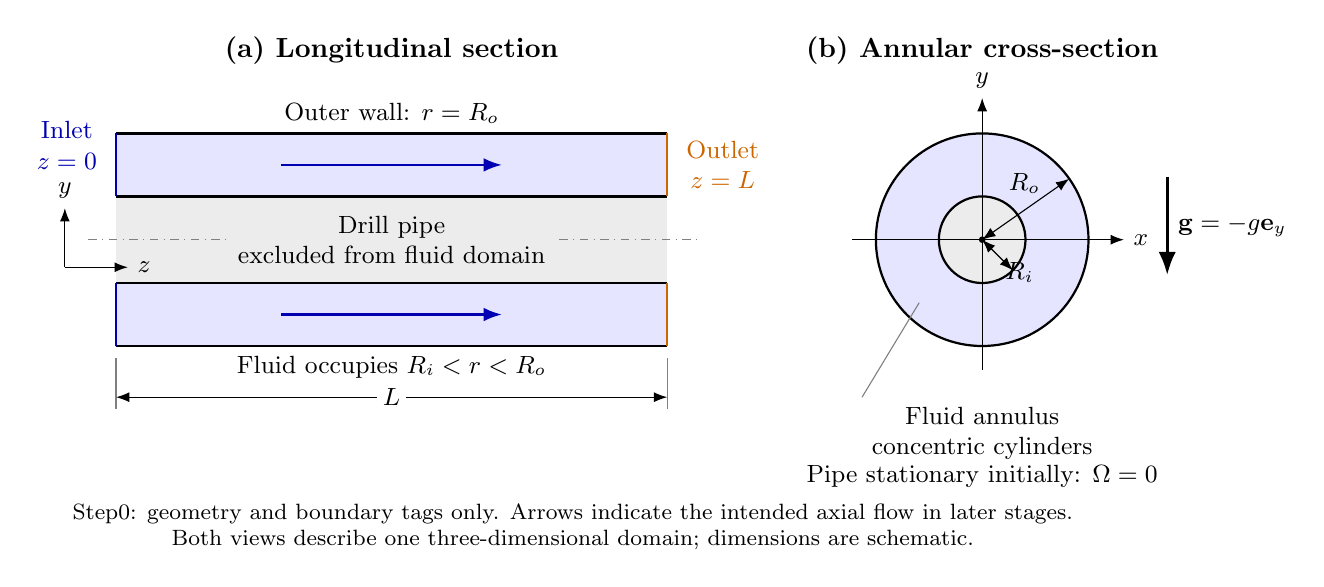
\begin{tikzpicture}[
        >=Latex,
        font=\small,
        wall/.style={thick},
        dimension/.style={<->,thin},
        guide/.style={thin,gray},
        flow/.style={->,thick,blue!70!black}
    ]

    % =========================================================
    % (a) Longitudinal section of the 3D annulus
    % Drawing dimensions are schematic, not physical values.
    % =========================================================
    \begin{scope}
        \def\Len{7}
        \def\Ro{1.35}
        \def\Ri{0.55}

        \node[font=\bfseries] at (3.5,2.4)
            {(a) Longitudinal section};

        % Fluid regions
        \fill[blue!10] (0,\Ri) rectangle (\Len,\Ro);
        \fill[blue!10] (0,-\Ro) rectangle (\Len,-\Ri);

        % Inner pipe: excluded from the fluid domain
        \fill[gray!15] (0,-\Ri) rectangle (\Len,\Ri);

        % Outer and inner cylindrical walls
        \draw[wall] (0,\Ro) -- (\Len,\Ro);
        \draw[wall] (0,-\Ro) -- (\Len,-\Ro);
        \draw[wall] (0,\Ri) -- (\Len,\Ri);
        \draw[wall] (0,-\Ri) -- (\Len,-\Ri);

        % Inlet and outlet sections (fluid portions only)
        \draw[thick,blue!70!black]
            (0,\Ri) -- (0,\Ro)
            (0,-\Ro) -- (0,-\Ri);
        \draw[thick,orange!80!black]
            (\Len,\Ri) -- (\Len,\Ro)
            (\Len,-\Ro) -- (\Len,-\Ri);

        % Axis
        \draw[dash dot,gray]
            (-0.35,0) -- (7.45,0);

        \node[align=center,fill=gray!15,inner sep=3pt]
            at (3.5,0)
            {Drill pipe\\excluded from fluid domain};

        % Prospective axial flow direction
        \draw[flow] (2.1,0.95) -- (4.9,0.95);
        \draw[flow] (2.1,-0.95) -- (4.9,-0.95);

        % Boundary labels
        \node[left,align=center,text=blue!70!black]
            at (-0.12,1.2) {Inlet\\$z=0$};
        \node[right,align=center,text=orange!80!black]
            at (7.12,0.95) {Outlet\\$z=L$};

        \node[above] at (3.5,\Ro)
            {Outer wall: $r=R_o$};

        \node[below] at (3.5,-\Ro)
            {Fluid occupies $R_i<r<R_o$};

        % Length dimension
        \draw[guide] (0,-1.5) -- (0,-2.15);
        \draw[guide] (\Len,-1.5) -- (\Len,-2.15);
        \draw[dimension] (0,-2.0) -- (\Len,-2.0)
            node[midway,fill=white,inner sep=2pt] {$L$};

        % Coordinate directions
        \draw[->] (-0.65,-0.35) -- (-0.65,0.4)
            node[above] {$y$};
        \draw[->] (-0.65,-0.35) -- (0.15,-0.35)
            node[right] {$z$};
    \end{scope}

    % =========================================================
    % (b) Cross-section normal to the z-axis
    % =========================================================
    \begin{scope}[shift={(11,0)}]
        \def\Ro{1.35}
        \def\Ri{0.55}

        \node[font=\bfseries] at (0,2.4)
            {(b) Annular cross-section};

        % Fluid annulus and excluded inner pipe
        \filldraw[fill=blue!10,wall]
            (0,0) circle (\Ro);
        \filldraw[fill=gray!15,wall]
            (0,0) circle (\Ri);

        % Centre
        \fill (0,0) circle (1.2pt);

        % Radius dimensions, at different angles
        \draw[dimension] (0,0) -- (35:\Ro)
            node[pos=0.70,above left,inner sep=1pt] {$R_o$};

        \draw[dimension] (0,0) -- (-45:\Ri)
            node[pos=0.65,below right,inner sep=1pt] {$R_i$};

        % Cartesian axes
        \draw[->] (-1.65,0) -- (1.8,0)
            node[right] {$x$};
        \draw[->] (0,-1.65) -- (0,1.8)
            node[above] {$y$};

        % Gravity
        \draw[->,very thick] (2.35,0.8) -- (2.35,-0.45)
            node[midway,right] {$\mathbf{g}=-g\mathbf{e}_y$};

        % Fluid label with leader
        \node[below,align=center] (fluidlabel) at (0,-2.0)
            {Fluid annulus\\concentric cylinders};
        \draw[guide] (fluidlabel.north west) -- (-0.8,-0.8);

        \node[align=center] at (0,-3)
            {Pipe stationary initially: $\Omega=0$};
    \end{scope}

    % Figure-wide note
    \node[align=center,font=\footnotesize] at (5.8,-3.65)
        {Step0: geometry and boundary tags only.
        Arrows indicate the intended axial flow in later stages.\\
        Both views describe one three-dimensional domain;
        dimensions are schematic.};

    \end{tikzpicture}
\end{document}
